\paragraph*{Events}
In order to better understand the remote server, it is necessary to identify the events that may occur, which are presented in table \ref{table:rs_events}.

\begin{table}[ht]
	\centering
	\resizebox{\columnwidth}{!}
	{
		\begin{tabular}{|m{3cm}|m{5cm}|m{2.4cm}|m{2.4cm}|}
			\hline
			\textbf{Event} & \textbf{System Response} & \textbf{Source} & \textbf{Type}\\
			\hline\hline
	
			Connection Request & Accept/ decline connection & Remote client & Asynchronous\\\hline
			
			Check Log-in Credentials & Validate username and pincode & Remote client (Mobile App) & Asynchronous\\\hline
			
			Add new lamppost & Add new lamppost info to \ac{db} & Remote client (Mobile App) & Asynchronous\\\hline
			
			Remove lamppost & Remove lamppost from \ac{db} & Remote client (Mobile App) & Asynchronous\\\hline
			
			Update lamppost information & Update lamppost info on \ac{db} & Remote client (Mobile App); Local System & Asynchronous\\\hline
			
			Check for lampposts with error status & Read and send lampposts with error status to Mobile App & Remote client (Mobile App) &  Asynchronous\\\hline
			
			Check for empty parking spots & Read and send available parking spots to Web Site & Remote client (Web Site) & Asynchronous\\\hline
		\end{tabular}
	}
	\caption{Events: Remote Server.}
	\label{table:rs_events}
\end{table}

\clearpage
\paragraph*{Use Cases}
The remote server use cases are shown in figure \ref{fig:UseCases_Server}. The remote(s) client(s) can interact with the remote server in various ways, as previously seen. This system only executes the demanded commands, from the remote clients or from the local systems, by accessing database information. The database interacts with the remote server by providing read, modify, remove or add register functions.

\begin{figure}[H]
	\centering
	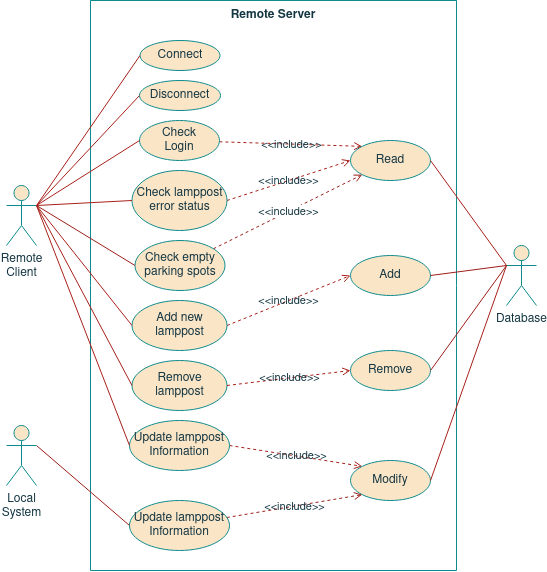
\includegraphics[width=1\textwidth]{06remote_system/Server_UseCases}
	\caption{Use Cases: Remote Server.}
	\label{fig:UseCases_Server}
\end{figure}

\paragraph*{State Chart}
In figure \ref{fig:StateChart_Server}, one can see the remote server state chart. After power on, the remote server does the system configuration, by initializing communication and database management services, and after that, the system executes concurrently these services until system's power off. These services give to the remote server the capability of processing received requests/commands, from the remote clients or from the local systems, and execute them, by accessing to database information.

\begin{figure}[H]
	\centering
	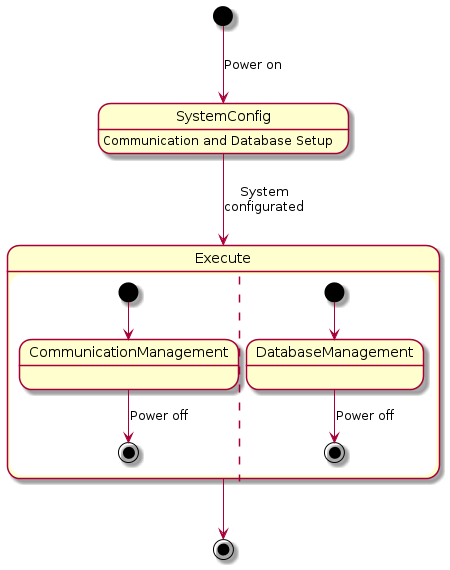
\includegraphics[width=0.8\textwidth]{06remote_system/Server_StateChart}
	\caption{State Chart: Remote Server.}
	\label{fig:StateChart_Server}
\end{figure}

\paragraph*{Sequence Diagram}
The sequence diagram of the remote server is shown in the figure \ref{fig:SeqDiagram_Server}. As seen previously, the remote client and the local system can execute several different actions. That is only possible if the remote server accepts the connection made from the remote client. After that, the remote server processes all received communications and, if needed, accesses the database to do so.

\begin{figure}[H]
	\centering
	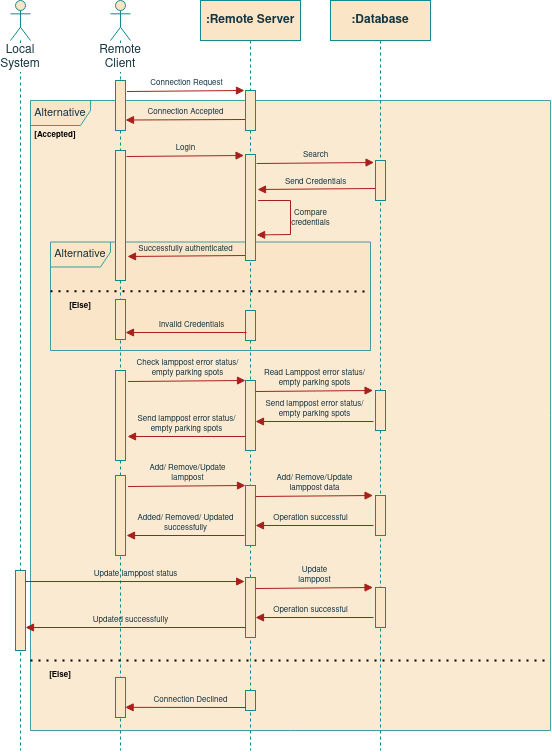
\includegraphics[width=1\textwidth]{06remote_system/Server_SeqChart}
	\caption{Sequence Diagram: Remote Server.}
	\label{fig:SeqDiagram_Server}
\end{figure}